\documentclass[a4paper]{article}

\usepackage[english]{babel}
\usepackage[utf8x]{inputenc}
\usepackage{amsmath}
\usepackage{graphicx}
\usepackage[colorinlistoftodos]{todonotes}
\usepackage{subfig}
\usepackage{float}


%_____________________________________________________________________________________
% THIS SOME THING THAT WILL GET OUR FIGURES IN THE RIGHT PLACE TAKEN FROM THE INTERNET ON THE WEBPAGE; http://mintaka.sdsu.edu/GF/bibliog/latex/floats.html

%%% START %%%
% Alter some LaTeX defaults for better treatment of figures:
    % See p.105 of "TeX Unbound" for suggested values.
    % See pp. 199-200 of Lamport's "LaTeX" book for details.
    %   General parameters, for ALL pages:
    \renewcommand{\topfraction}{0.9}	% max fraction of floats at top
    \renewcommand{\bottomfraction}{0.8}	% max fraction of floats at bottom
    %   Parameters for TEXT pages (not float pages):
    \setcounter{topnumber}{2}
    \setcounter{bottomnumber}{2}
    \setcounter{totalnumber}{4}     % 2 may work better
    \setcounter{dbltopnumber}{2}    % for 2-column pages
    \renewcommand{\dbltopfraction}{0.9}	% fit big float above 2-col. text
    \renewcommand{\textfraction}{0.07}	% allow minimal text w. figs
    %   Parameters for FLOAT pages (not text pages):
    \renewcommand{\floatpagefraction}{0.7}	% require fuller float pages
	% N.B.: floatpagefraction MUST be less than topfraction !!
    \renewcommand{\dblfloatpagefraction}{0.7}	% require fuller float pages

	% remember to use [htp] or [htpb] for placement
    
%%% END %%%
%_____________________________________________________________________________________

% NEEDED FOR THE REFERENCE
 %_______SOURCE; 

% START
\usepackage{hyperref}
% END


% NEEDED FOR SOURCE CODE (JAVA) TO FUNCTION NICELY
% SOURCE; http://stackoverflow.com/questions/3175105/how-to-insert-code-into-a-latex-doc
%START
\usepackage{listings}
\usepackage{color}
\definecolor{dkgreen}{rgb}{0,0.6,0}
\definecolor{gray}{rgb}{0.5,0.5,0.5}
\definecolor{mauve}{rgb}{0.58,0,0.82}

\lstset{frame=tb,
  language=Java,
  aboveskip=3mm,
  belowskip=3mm,
  showstringspaces=false,
  columns=flexible,
  basicstyle={\small\ttfamily},
  numbers=none,
  numberstyle=\tiny\color{gray},
  keywordstyle=\color{blue},
  commentstyle=\color{dkgreen},
  stringstyle=\color{mauve},
  breaklines=true,
  breakatwhitespace=true,
  tabsize=3
}
%END





\title{Design and Control of a Lego Unicycle}
\author{Group B: Johan Kellerth Fredlund | Koshin Aliabase\\ Santiago Castro Chans | Sadik Kenan Sulejmanovic}

\begin{document}
\maketitle

\begin{abstract}
Your abstract.
\end{abstract}

\tableofcontents

\section{Author's note}

\section{Introduction}

We are designing a unicycle made by lego with an integrated inertia wheel to keep the lateral balence. The project therefore consists of two problems. To stabilize the unicycle in the medial direction by designing a controller for the ground wheel, and to stabilize it in the lateral direction by applying a reaction wheel connected to the top of the unicycle.

\section{Construction}

	\subsection{Ev3}
	The EV3 is the third generation of Lego Mindstorms platforms, the specification of this platform can be seen in the table \ref{table:spec_ev3}. Furthermore some options for programming platforms are listed in the table \ref{table:prog_platforms_ev3}. Lastly can a picture of the EV3 also be seen in figure \ref{fig:ev3_platform_picture}
	
	 \begin{table}[h]
		\center
		\begin{tabular}{|c |c|}
			\hline
			 Processor &  ARM9   \\ 
			\hline
			OS   & Linux- based  \\ 
			\hline
			Sensor ports & 4 , analog, digital (up to 460.8 Kbit/sec)  \\
	        		\hline
			Motor port & 4, with encoders \\
			\hline
			SD- card & Micro SD- Card Reader, (up to 32 GB)   \\
			\hline
		\end{tabular}
		\caption{Specifications for the EV3 platform found at \cite{EV3spec}.}
		\label{table:spec_ev3}
	\end{table}
	
	 \begin{table}[h]
		\center
		\begin{tabular}{|c|}
			\hline
			Programing platforms   \\ 
			\hline
			Lejos (extension of JAVA)  \\ 
			\hline
			RobotC (similar to C) \\
	        		\hline
			NCX (similar to C )\\
			\hline
		\end{tabular}
		\caption{Some of the optional programing platforms for the EV3.}
		\label{table:prog_platforms_ev3}
	\end{table}
	
	
	
		\begin{figure}[h]
		\centering
		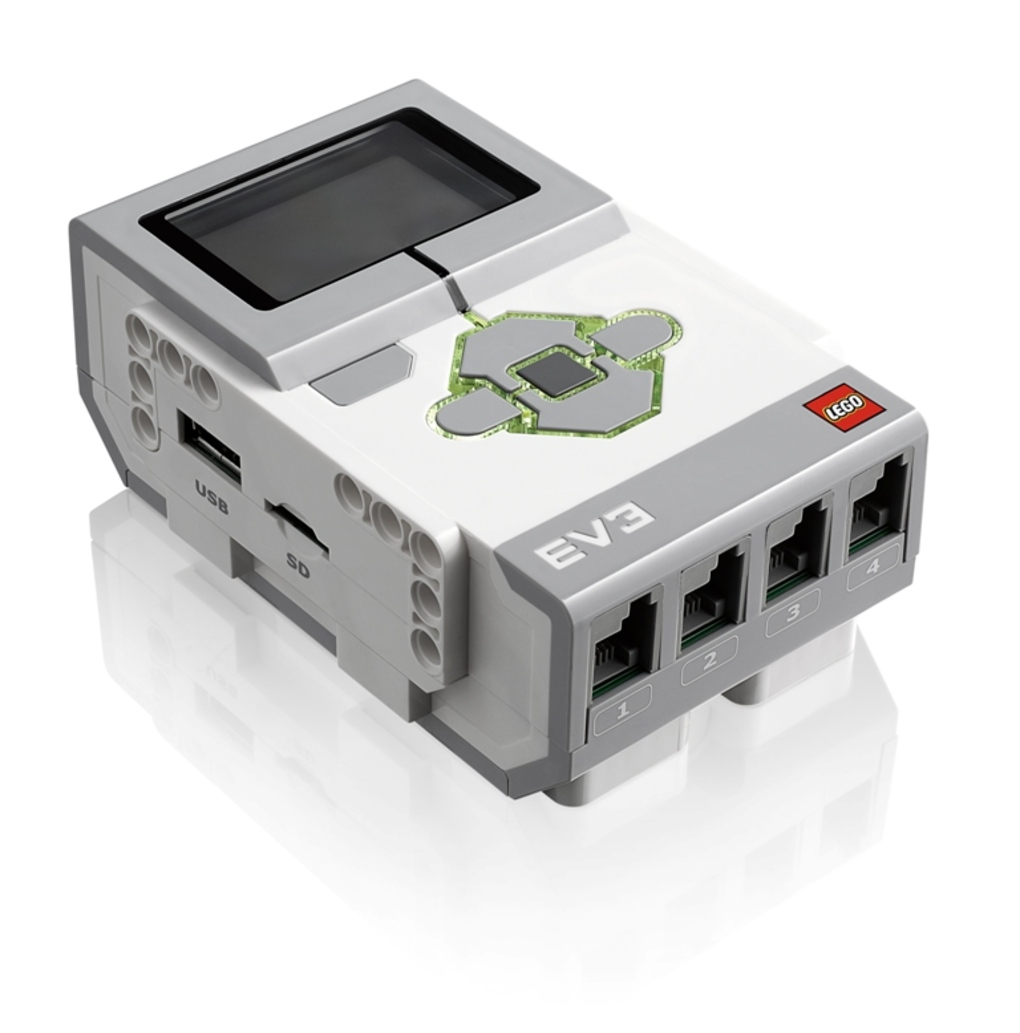
\includegraphics[width=0.2\textwidth,height=0.2\textheight]{ev3_platform}
		\caption{Shows how the hardware platform EV3 looks like which was used in the project.}
		\label{fig:ev3_platform_picture}
	\end{figure}
	
	
	
	
    \subsection{Sensors}
    	\subsubsection{HighTechinic Gyro Sensor}
        The Gyro sensor gives the rate of change in x, y and z orientation in radians per second. More specified details about the sensor can be seen in the table \ref{table:Gyro_sensor}. The first row shows how long time it takes for our program to fetch a sample, second row shows how accurate the sensor is given by specification by the manufacturer and the last line shows the update time of the sensor also given by the manufacturer. 
\\In nature all gyroscopes has a drift and offset, both are unwanted. The drift means that the rate of change will increase with time even though the sensor is stationary as can been observed in the figure \ref{fig:Gyro_offsets_refresh_times}. Secondly the offset is the property that give a constant value although the sensor is stationary. How we dealt with these problems will be explained in later sections. Lastly can we see the gyro sensor in figure \ref{fig:NXT_Gyro_Sensor}.  
        
        
        % THE TABLE DESCRIBING THE PROP. of the gyro sensor
        \begin{table}[h]
		\center
		\begin{tabular}{|c |c|}
			\hline
			 Refresh time in program & 10 ms (average)   \\ 
			\hline
			Accuracy &  $\pm 1$ degree \cite{NXT_Gyro_Sensor} \\ 
			\hline
			Update of value & 300 times / second  \cite{NXT_Gyro_Sensor} \\
	        		\hline
		\end{tabular}
		\caption{Specifications for the gyro under the name NXT Gyro Sensor (NGY1044).}
		\label{table:Gyro_sensor}
	\end{table}


	\begin{figure}[h]
		\centering
		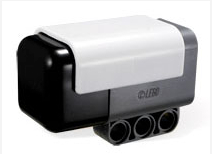
\includegraphics[width=0.3\textwidth]{NXT_Gyro_Sensor}
		\caption{Shows the gyro sensor which was used in the project.}
		\label{fig:NXT_Gyro_Sensor}
	\end{figure}
	
	\begin{figure}[h]
		\centering
		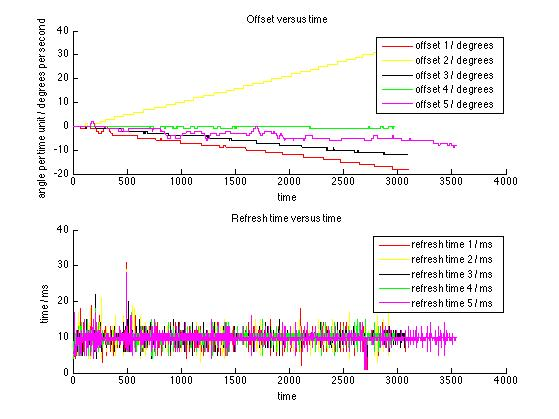
\includegraphics[width=1.3\textwidth]{plot_gyro_test_final_20150107}
		\caption{Shows the gyro sensor's offsets and refresh times when beeing stationary.}
		\label{fig:Gyro_offsets_refresh_times}
	\end{figure}
	
	\newpage
        
        
        \subsubsection{HighTechinic Accelerometer Sensor}
        
The accelerometer measure acceleration in x, y and z direction relative to the sensors specified directions given by the manufacturer. The specifications of the accelerometer can be seen in the table \ref{table:Acce_sensor} which shows the the time for it to give a sample to our program respectively number of times the sensor can update a value. On the other hand this sensor also comes with unwanted properties which is that the value is (very) noise however when it is not noise it gives reasonable good data. We can also see how this sensor looks like in the figure \ref{fig:NXT_Acce_Sensor} and the refresh time for a longer of time can be seen in the figure \ref{fig:plot_acce_refresh_time}
         % THE TABLE DESCRIBING THE PROP. of the Acce sensor
         \begin{table}[h]
		\center
		\begin{tabular}{|c |c|}
			\hline
			 Refresh time in program & 20 ms (average)   \\ 
			\hline
			Update of value &  100 times / second \cite{NXT_Acce} \\ 
			\hline
		\end{tabular}
		\caption{Specifications for the accelerometer under the name NXT Acceleration (NAC1040).}
		\label{table:Acce_sensor}
	\end{table}
	
	\begin{figure}[h]
		\centering
		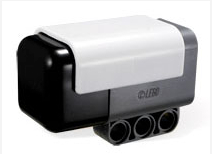
\includegraphics[width=0.3\textwidth]{NXT_Gyro_Sensor}
		\caption{Shows the accelerometer sensor which was used in the project.}
		\label{fig:NXT_Acce_Sensor}
	\end{figure}
	
	\begin{figure}[h]
		\centering
		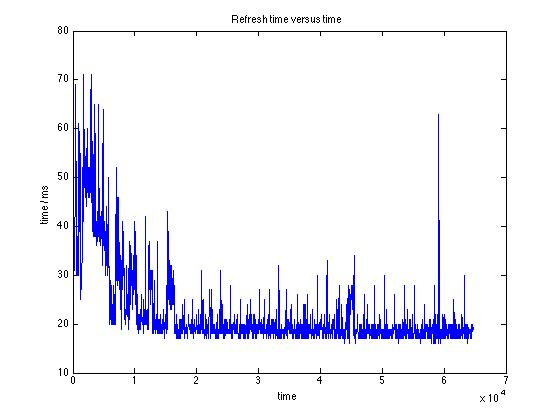
\includegraphics[width=1.3\textwidth]{plot_acce_refresh_time_20150107}
		\caption{Shows the accelerometer sensor refresh time.}
		\label{fig:plot_acce_refresh_time}
	\end{figure}
	
	
         
        
        
        \subsubsection{AbsoluteIMU-ACG}
        The AbsoluteIMU-ACG can gives gyro, accelerometer and compass data but in this project we are only interested in the gyro and the accelerometer therefor we will only discuss those measurements. As discussed previously gives the gyro part the rate of change in x,y and z. The accelerometer part measures the gravity in the x,y and z direction. The interesting part of this sensor is the refresh time versus the previous sensors and the update time can be seen in the figure \ref{fig:plot_IMU_sensor_sensitivity_0}. With this sensor one can also choose to have a smoothing filter for the accelerometer part of the IMU, downside is that this will increase the refresh time of the sensor. Therefor we did two measurements, one with sensitivity 0 and one with sensitivity 4 (figure \ref{fig:plot_IMU_sensor_sensitivity_4}). 
        
        \begin{figure}[h]
		\centering
		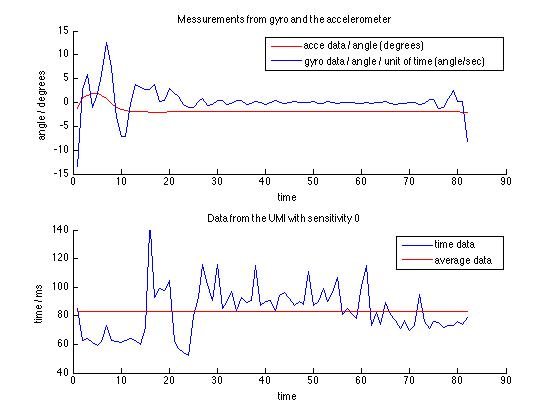
\includegraphics[width=1.3\textwidth]{plot_data_UMI_sen_0_20150103}
		\caption{Shows the important properties of the IMU sensor with sensitivity 0.}
		\label{fig:plot_IMU_sensor_sensitivity_0}
	\end{figure}
	
	      \begin{figure}[h]
		\centering
		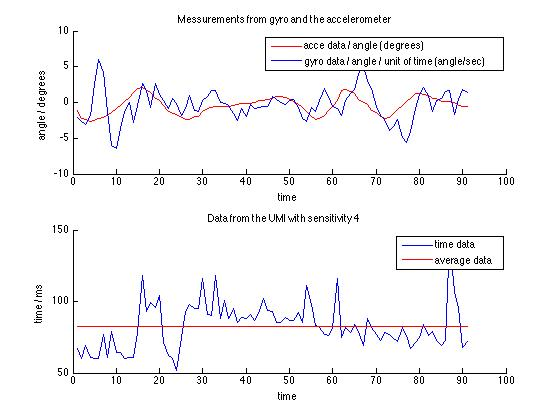
\includegraphics[width=1.3\textwidth]{plot_data_UMI_sen_4_20150107}
		\caption{Shows the important properties of the IMU sensor with sensitivity 4.}
		\label{fig:plot_IMU_sensor_sensitivity_4}
	\end{figure}
	
	
	\begin{table}[h]
		\center
		\begin{tabular}{|c |c|}
			\hline
			 Refresh time in program &  83 ms (average)   \\ 
			\hline
			Update of value &  100 times / second  \cite{IMU_sensor} \\ 
			\hline
		\end{tabular}
		\caption{Specifications for the IMU-ACG sensor.}
		\label{table:IMU_sensor}
	\end{table}
	
        
        
    \newpage 
    \subsection{Reaction wheel}
    
    The reaction wheel modeling is explained in the section \ref{sec:Modeling} and some conclusion can be drawn from that. In this section we will bring up what those conclusion became in reality. Because we want as much weight as possible in the outer ring so nuts screwed in the material was the obvious choice. The choice of material was between plastic and wood, because of the nature of time and availability of personal it became wood. Plastic was preferable wood would also make it work. Due to the heavier weight of wood due to its nature it became a problem but was solved with making circles in the circle of wood so the most of the weight was taken out but leave enough for the circle not to crack under pressure of acceleration. The end product of the reaction wheel can be seen in the figure \ref{fig:reaction_wheel_end_product} while the dimensions is shown in the table \ref{table:spec_reaction_wheel}. Meanwhile the design of the initial reaction wheel be seen in the figure \ref{fig:reaction_wheel_initial_design}. Thirdly is wort mentioning that the wholes at the end of the circle in figure \ref{fig:reaction_wheel_initial_design} is for the nuts to go in and the cross in the middle is for the attachment to the axis going to the EV3 Large Servo Motor. More on this topic under the section \ref{sec:Attachment_reaction_wheel_EV3_Motor}
    
    
       \begin{figure}[h]
		\centering
		\includegraphics[width=0.5\textwidth,height=0.5\textwidth]{reaction_wheel_initial_design}
		\caption{Shows the initial design for the reaction wheel.}
		\label{fig:reaction_wheel_initial_design}
	\end{figure}
	
	
	\begin{table}[h]
		\center
		\begin{tabular}{|c |c|}
			\hline
			Diameter & 30 cm    \\ 
			\hline
			Thickness & 8 mm  \\ 
			\hline
		\end{tabular}
		\caption{Shows the dimensions of the end product of the reaction wheel.}
		\label{table:spec_reaction_wheel}
	\end{table}
	
      \begin{figure}[h]
		\centering
		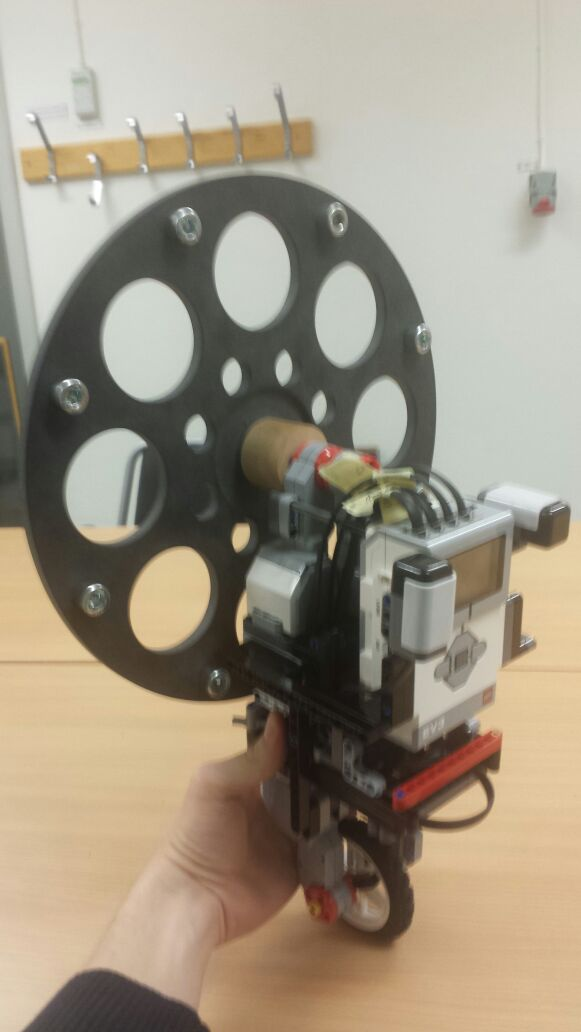
\includegraphics[width=0.7\textwidth,height=0.7\textwidth]{reaction_wheel_endproduct_picture}
		\caption{Shows the end product of the reaction wheel with the whole prototype at one stage.}
		\label{fig:reaction_wheel_end_product}
	\end{figure}
    
    
    
    
    
    
    
    
    \newpage
 \subsubsection{Attachment between the reaction wheel and EV3 Large Motor } 
 \label{sec:Attachment_reaction_wheel_EV3_Motor}
 
 Due to the attachment of the sensors on the current prototype we build in one small circular block to the reaction wheel which also had wholes matching the attachment directly to the EV3 Motor attachment. The specific attachment pattern is shown in figure \ref{fig:pattern_EV3_attachment}. By using that specific pattern we achieved more stability of the reaction wheel but still there were problems with leaning of the reaction wheel relative to the full scale prototype. We also experienced wobbling of the reaction wheel when it was set to use. Therefore we rebuild the reaction wheel once more relative to the initial design with one more circular block on the other side of the reaction wheel which meant that we now had two circular blocks coming out from the reaction wheel at both ends. The prototype holding up the reaction wheel was also rebuild due to rebuilding of the reaction wheel, more on rebuilding of the full prototype can be seen in section \ref{sec:Prototypes}. Thus in the end leading to a full stable reaction wheel relative to the full scale prototype. The end attachment of the reaction wheel is shown in figure \ref{fig:reaction_wheel_attachment_end_product}
 
    \begin{figure}[h]
		\centering
		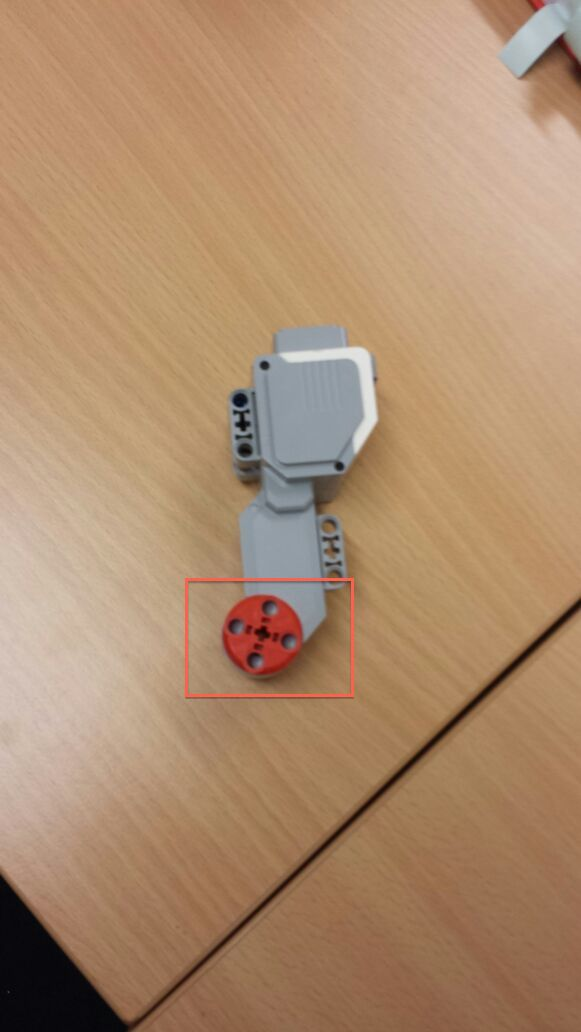
\includegraphics[width=0.3\textwidth]{attachment_pattern_EV3_Large_Motor}
		\caption{The red rectangle specifies the attachment pattern on the EV3 motor.}
		\label{fig:pattern_EV3_attachment}
	\end{figure}


	
	    \begin{figure}[h]
		\centering
		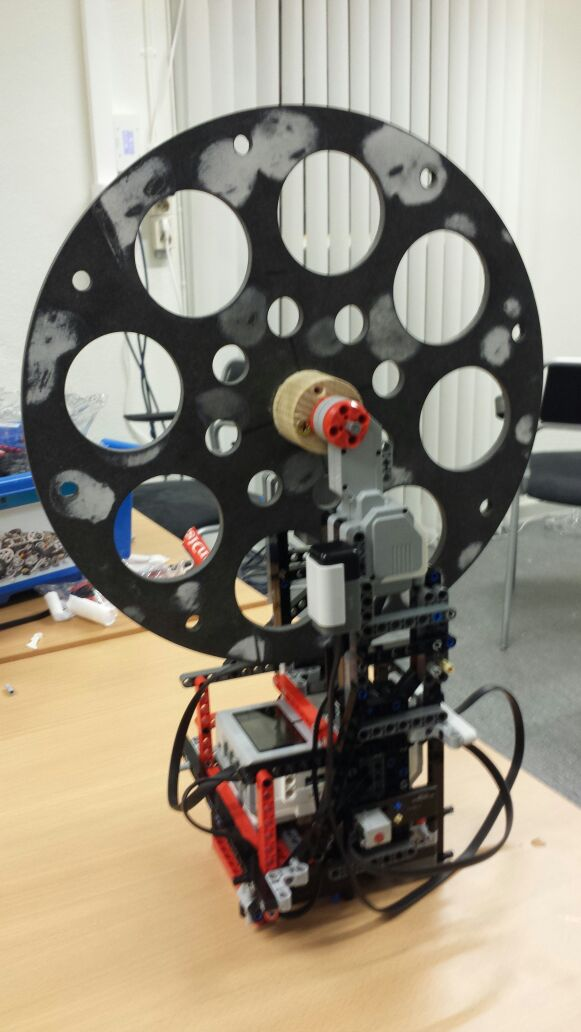
\includegraphics[width=0.5\textwidth,height=0.5\textheight]{reaction_wheel_attachment_end_product}
		\caption{Shown the end product of the attaching of the reaction wheel with the two engines.}
		\label{fig:reaction_wheel_attachment_end_product}
	\end{figure}
	
 
    \newpage
    \subsection{Motors}
    	\subsubsection{EV3 Large Servo Motor}
	\label{sec:EV3 Large Servo Motor}
	This is one of the strongest motors there is for LEGO and the specifications for this motor can be seen in the table 	  \ref{table:EV3_Large_servo_motor}. One experiment was done to get the connection between the torque and the power which is the parameter that control the PWM that goes to the motor. The power goes from -100 to 100. The result can be seen in the figure \ref{fig:plot_power_torque}.
    
 
       \begin{figure}[h]
		\centering
		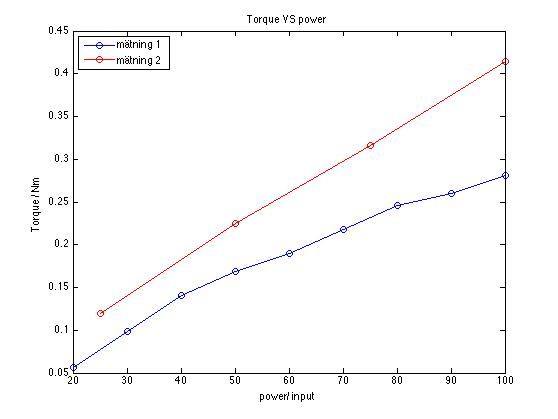
\includegraphics[width=1.3\textwidth]{plot_torque_versus_power_20151207}
		\caption{Shows the relation between the power and the torque of the motor.}
		\label{fig:plot_power_torque}
	\end{figure}
	
	\begin{table}[h]
		\center
		\begin{tabular}{|c |c|}
			\hline
			 RPM &  160 - 170  \cite{Ev3_Large_Servo_Motor}  \\ 
			\hline
			Running torque &  20 N/cm \cite{Ev3_Large_Servo_Motor}  \\ 
			\hline
			Stall torque  &  40 N/cm  \cite{Ev3_Large_Servo_Motor}  \\
			\hline
		\end{tabular}
		\caption{Specifications for the EV3 large motor server.}
		\label{table:EV3_Large_servo_motor}
	\end{table}
	
	
    
    \newpage
    \subsection{Prototypes}
    \label{sec:Prototypes}
In this section we will bring up the limitations of the physical construction of the lego segway and bring up some key limitations of the model as well. \\The most critical limitations is the building blocks of Lego because of some key concepts. The first being that the attachment pieces which holds the lego blocks together are not the most stable one which means that is you put two blocks together you can not expect that the blocks are held together while have some stress on them. They will fold not all the way by enough for the prototype to experience wobbles when the reaction wheel starts to accelerate and move around. This problem was experienced with great signification in the three first prototypes but the last one held it out pretty well considering that the system was made in lego. 

The second limitation is availability of the connection points on the EV3, there are some but could be more of them. From a building perspective this set great boundaries on how you might build your prototype hence the four prototypes. Each of them had strengths and weaknesses which is brought up in the table \ref{table:prototype_properties}. The possible options that the different categories can be are shown in the table \ref{table:def_prototypes}, these options are taken up to give a hint of how the different prototypes act when used and are therefore not scientific in a since that you can measure them. 

 
    
    
 
    \begin{figure}[h]
	\subfloat[]{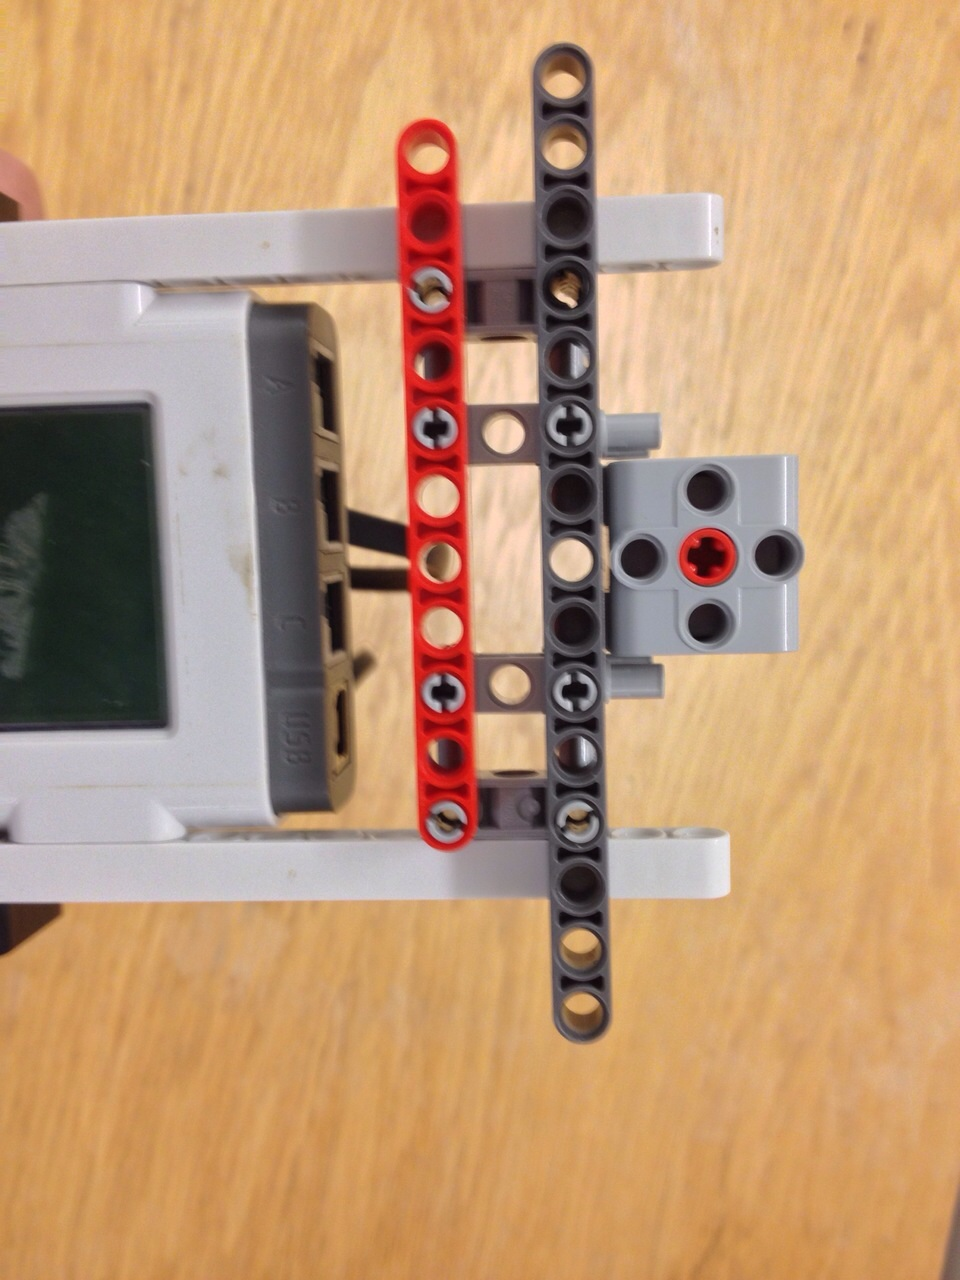
\includegraphics[width=0.3\textwidth,height=0.2\textheight]{prototype_1_a}} 
	\subfloat[]{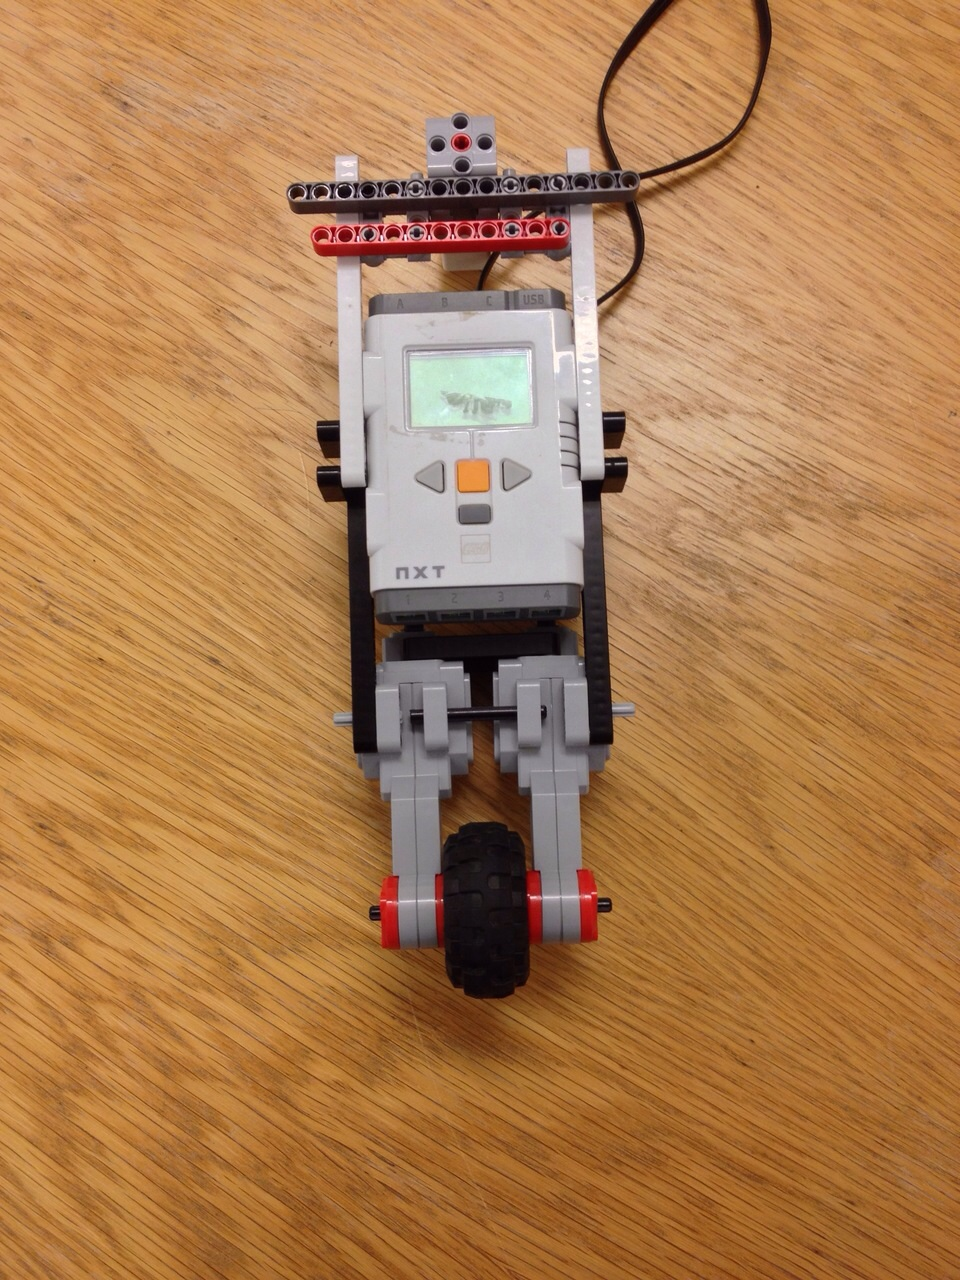
\includegraphics[width=0.3\textwidth,height=0.2\textheight]{prototype_1_b}} 
	\subfloat[]{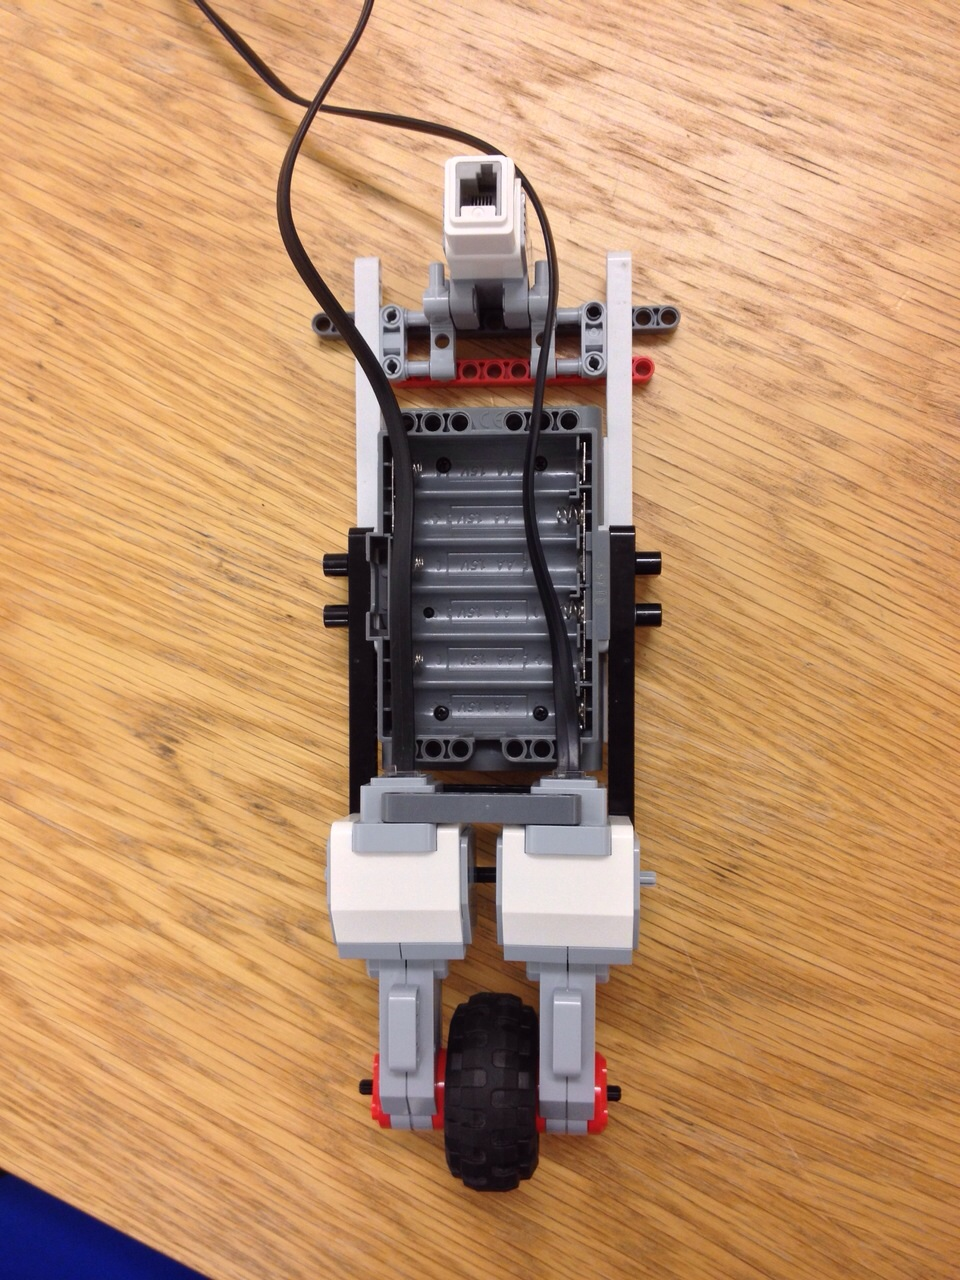
\includegraphics[width=0.3\textwidth,height=0.2\textheight]{prototype_1_c}}  \\
	\subfloat[]{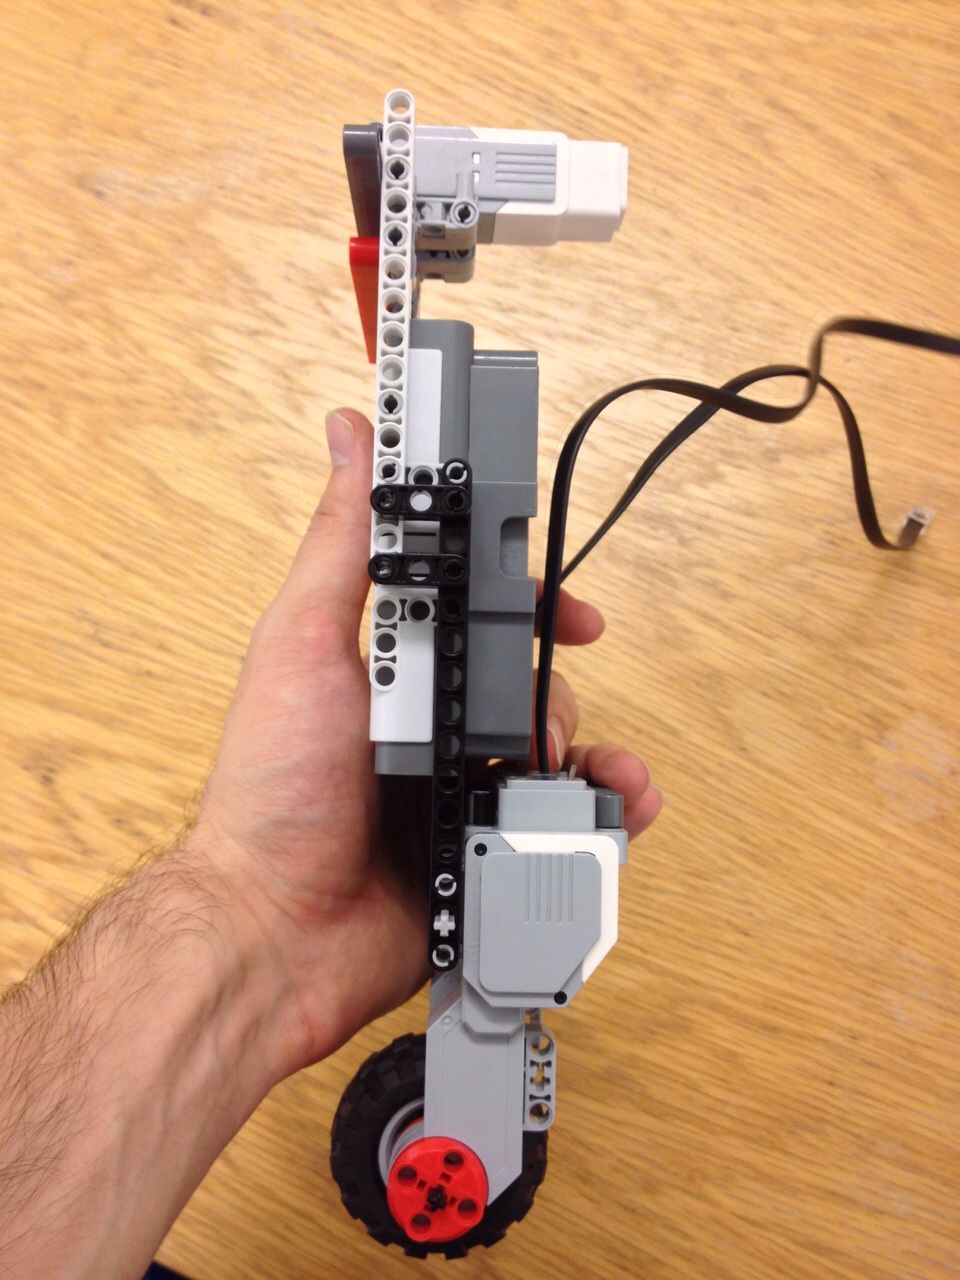
\includegraphics[width=0.3\textwidth,height=0.2\textheight]{prototype_1_d}} 
	\subfloat[]{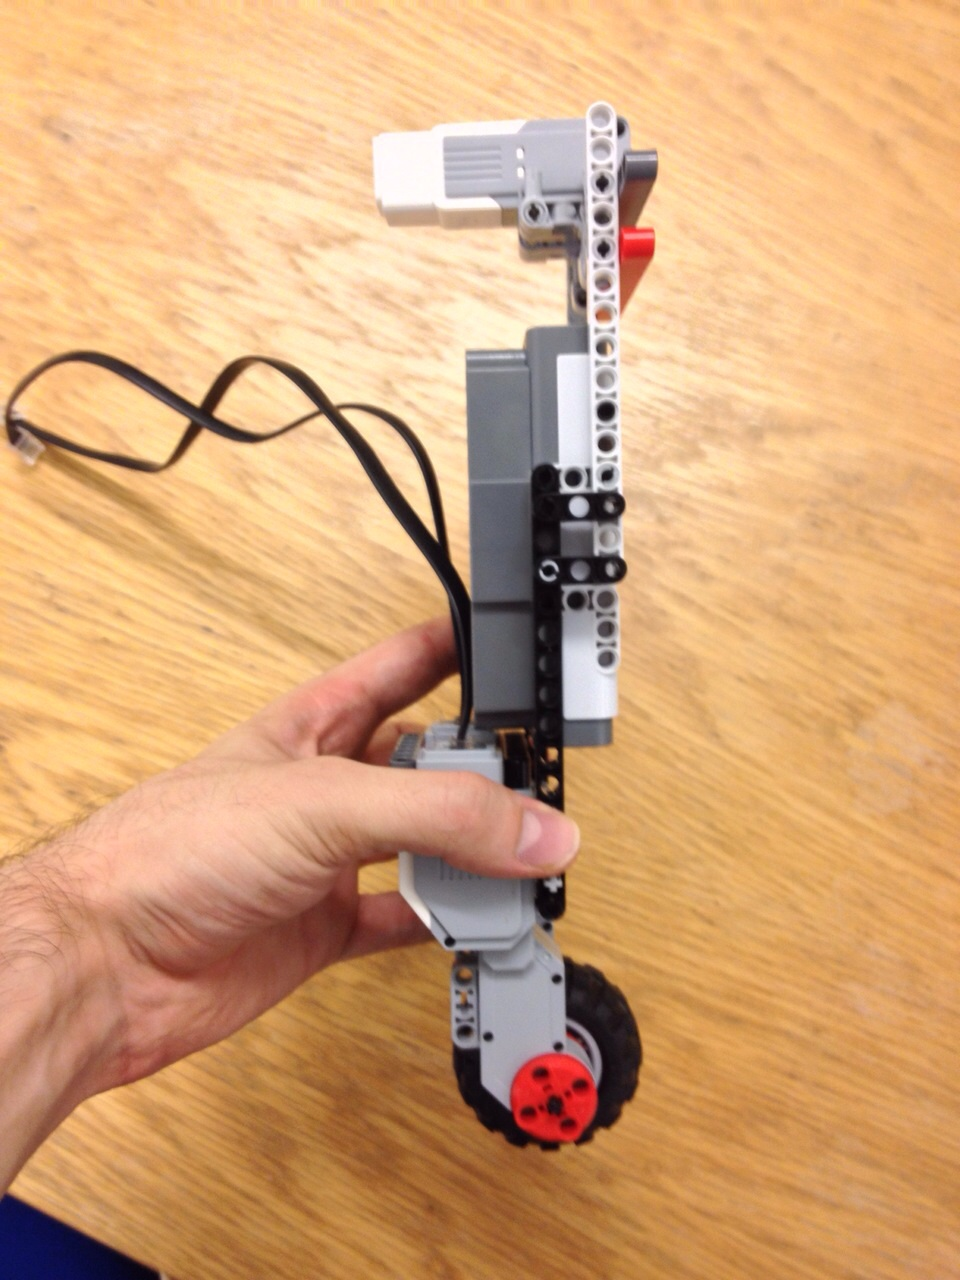
\includegraphics[width=0.3\textwidth,height=0.2\textheight]{prototype_1_e}} 
	\subfloat[]{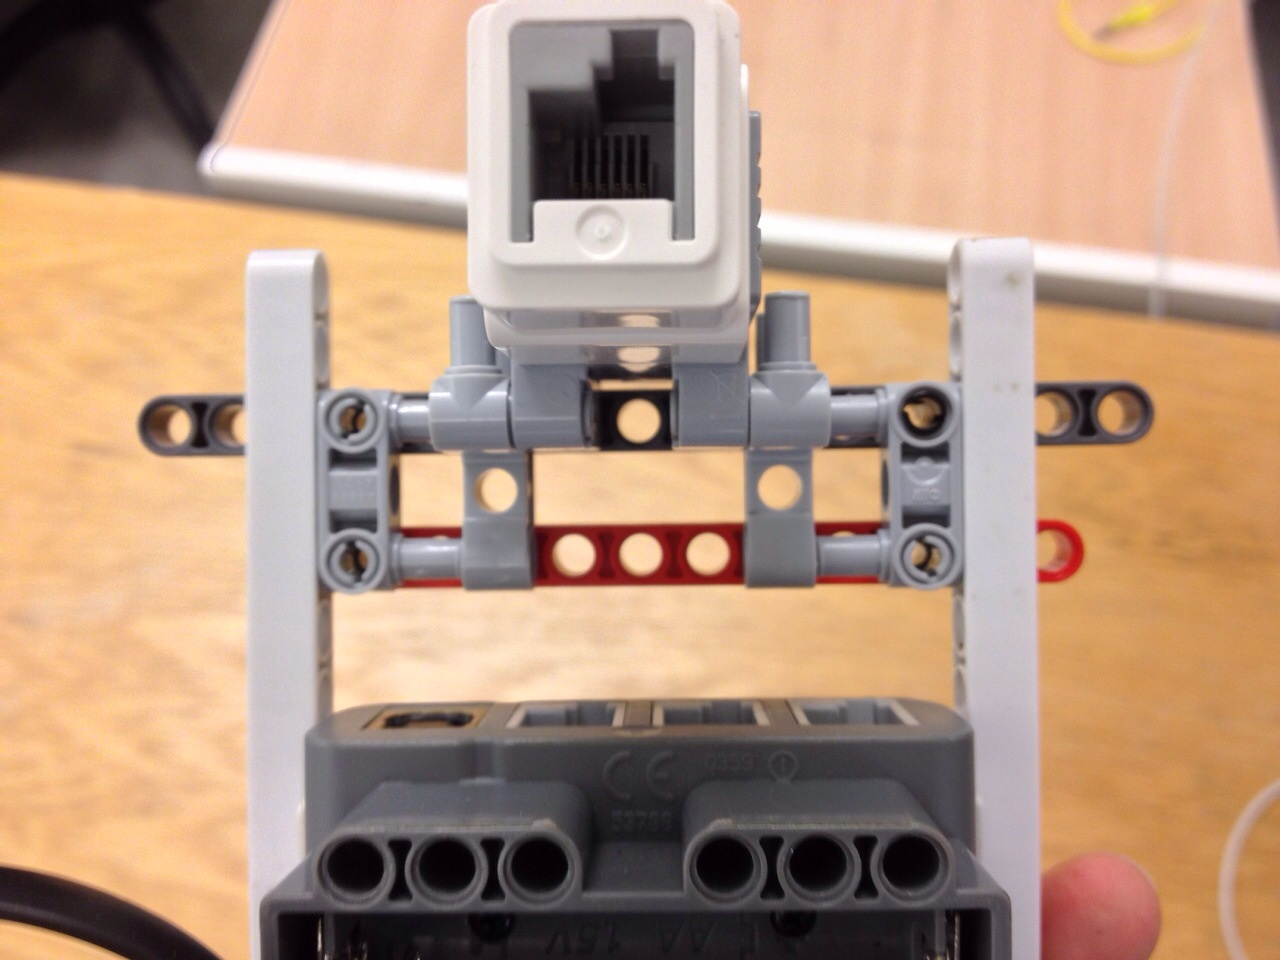
\includegraphics[width=0.3\textwidth,height=0.2\textheight]{prototype_1_f}}
	\caption{Shows the first prototype from different angles.}
    \end{figure}
    
    \begin{table}[h]
		\begin{tabular}{|c |c| |c|  |c|  |c|  }
			\hline
			Categories & p1 & p2 & p3 & p4	\\
			\hline
			 Handle stress due to reaction wheel  & - & falling apart & bad &  good \\ 
			\hline
			Stationary movement &  - &  forward & weak forward & stationary \\ 
			\hline
			Gravidation centre  &  middle  & high & high & low \\
			\hline
			Reaction wheel torn out  & - & yes & yes & no \\
			\hline
		\end{tabular}
		\caption{The prototype properties for different categories, where pN is as follows; the p for prototype and the N for which one (e.g. p1 stands for prototype 1)."-" means that is was never tested.}
		\label{table:prototype_properties}
	\end{table}
	
	
	\begin{table}[h]
		\begin{tabular}{|c |c|   }
			\hline
			Categories & The possible options	\\
			\hline
			 Handle stress due to reaction wheel  & falling apart-bad-magageable-good \\ 
			\hline
			Stationary movement &  falling forward-falling backward-stationary\\ 
			\hline
			Gravidation centre  & low-middle-high \\
			\hline
			Reaction wheel torn out  & yes-no \\
			\hline
		\end{tabular}
		\caption{The different options that the categories can take in the table \ref{table:prototype_properties}.}
		\label{table:def_prototypes}
	\end{table}

    
    
    
    \begin{figure}[h]
	\subfloat[]{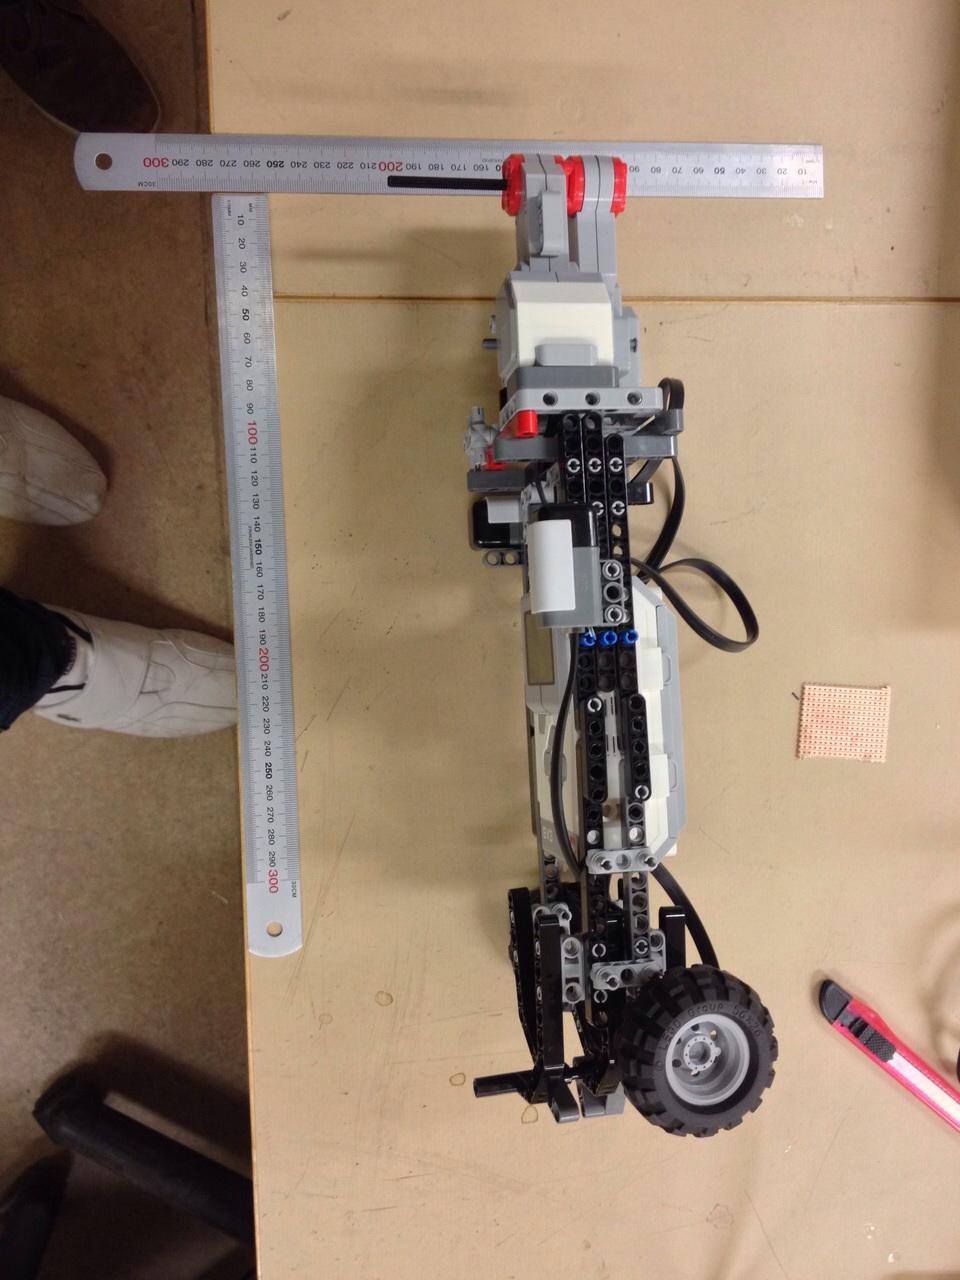
\includegraphics[width=0.35\textwidth,height=0.25\textheight]{prototype_2_a}} 
	\subfloat[]{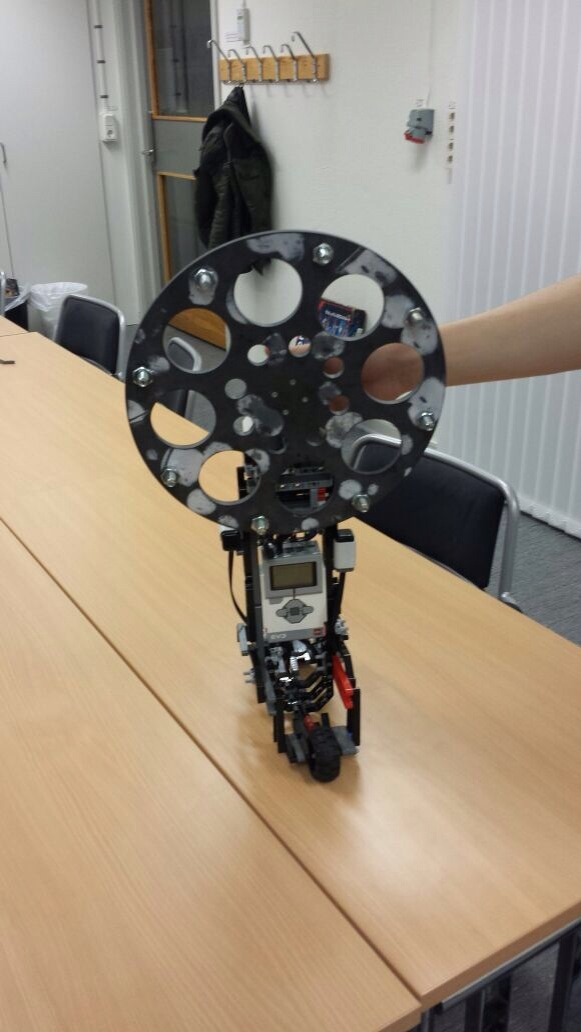
\includegraphics[width=0.35\textwidth,height=0.25\textheight]{prototype_2_b}} 
	\subfloat[]{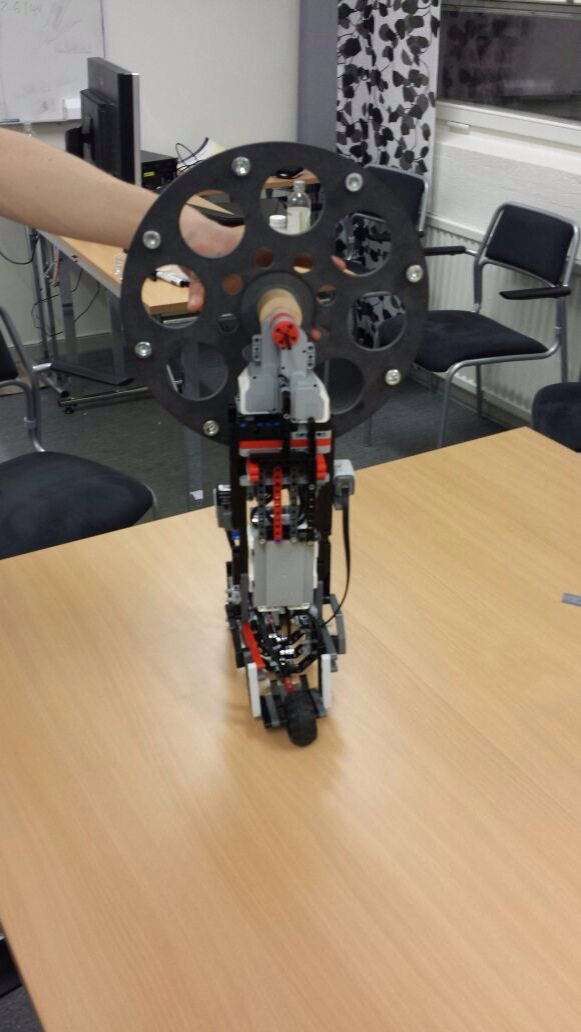
\includegraphics[width=0.35\textwidth,height=0.25\textheight]{prototype_2_c}}  
	\caption{Shows the second prototype from different angles with the first prototype of the reaction wheel.}
    \end{figure}
    
        \begin{figure}[h]
        \center
	 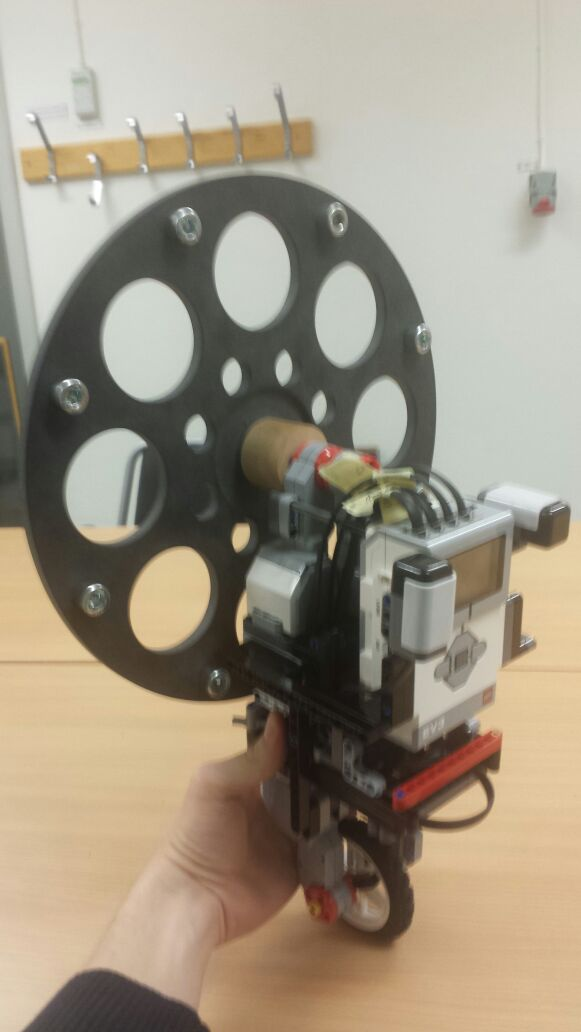
\includegraphics[width=0.5\textwidth,height=0.5\textheight]{prototype_3_a}
	\caption{Shows the third prototype with the first prototype of the reaction wheel.}
    \end{figure}
    
      \begin{figure}[h]
      	\center
	\subfloat[]{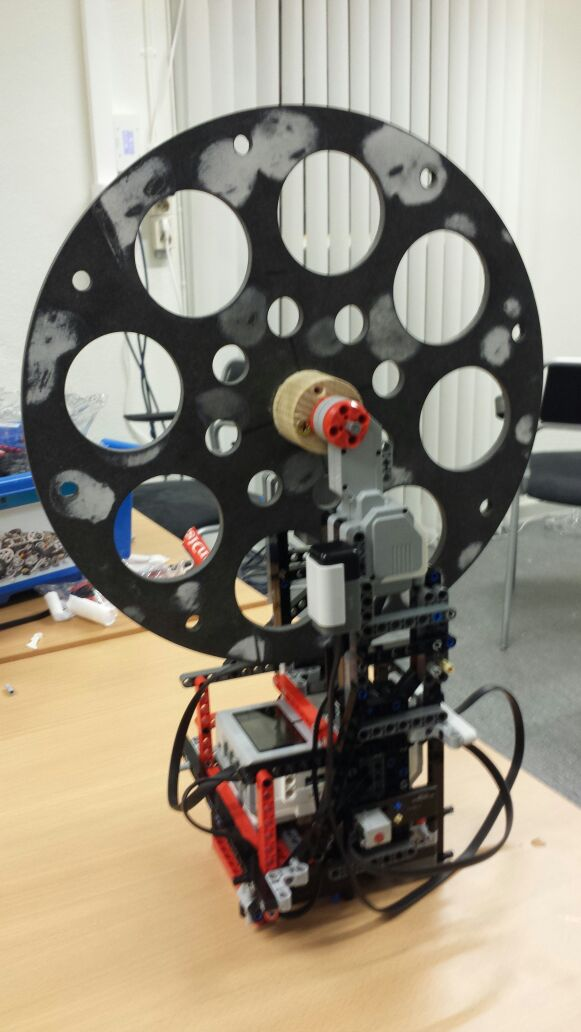
\includegraphics[width=0.35\textwidth,height=0.30\textheight]{prototype_4_a}} 
	\subfloat[]{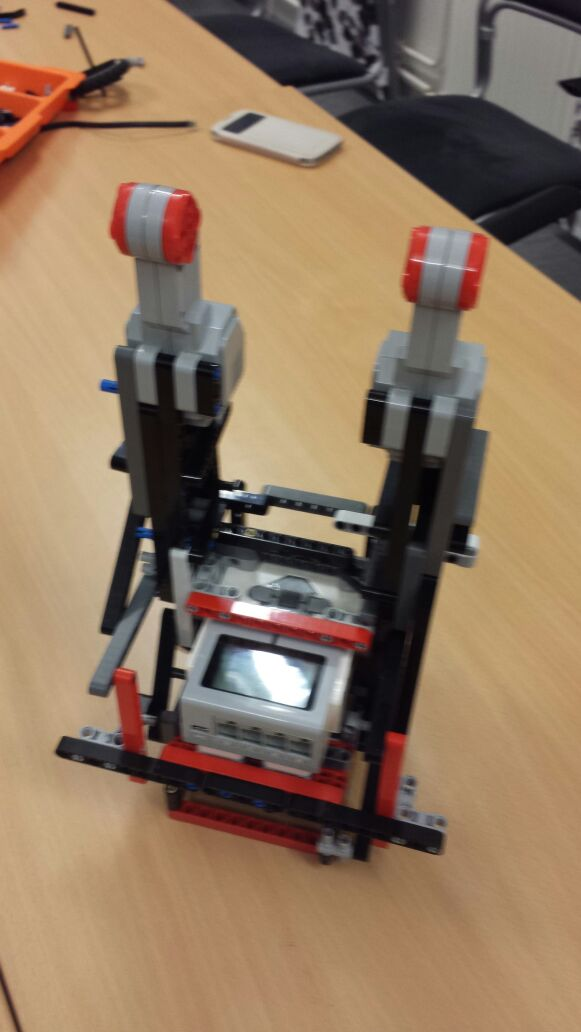
\includegraphics[width=0.35\textwidth,height=0.30\textheight]{prototype_4_b}} 
	\caption{Shows the fourth prototype from different angles with the first prototype of the reaction wheel.}
    \end{figure}
    
    
    
    
    
    
    
    
    
\newpage

\clearpage

\section{Modeling}
\label{sec:Modeling}
	\subsection{Lateral Balance}
	
	We realized early in the project that controlling the inertia wheel is the most complicated part of the project. The complexity comes from several areas. The sensors have to be very accurate (which they are not), the simulation in simulink had to take account of the relationship between torque and the speed of the wheel among other things, we had to design a working controller.

The unicycle is similar to an inverted pendulum with a point mass in the center of mass, with an additional mass that is the inertia wheel, seen in figure 17. We modelled the pendulum as can be seen in (1). The relevant states from the model are the angle of the pendulum, the the angular velocity of the pendulum and the angular velocity of the inertia wheel. The angular position of the inertia wheel is not important as only the change in angular position affects the torque. Torque is the momentum you get when a vector force is acted on the wheel with a certain radius. The torque acting on the pendulum due to gravity (which makes it fall) must be less that the torque from the inertia wheel (which we can control) for it to be stable. The reaction torque is therefore dependent on the radius of the wheel. The maximum torque of the engine is also limited, so some angles are impossible for the reaction wheel to stabilize.

To optimize the controller we implemented a linear quadratic regulator which minimizes the cost function, seen in (2). The Q matrix determines how much each state will be penalized. Since we want to keep cost function (J) small a large Q will require that the states are small. Q=[q1 0 0; 0 q2 0; 0 0 q3].

\begin{figure} [h]
	\centering
	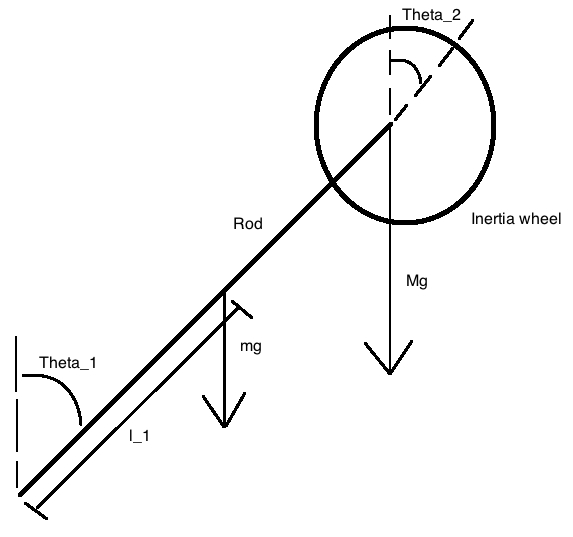
\includegraphics[width=0.7\textwidth]{Inverted_pedulum_2}
	\caption{Shows the sketch of the inverted pendulum}
	\label{fig:sketch_inverted_pendulum}
\end{figure}

\newpage	
	
		\subsubsection*{Mathematical model}
		
The principle idea of this control problem is to receive a reaction torque from 			the inertia wheel that is larger than the torque exerted on the unicycle from 				gravity. Looking at figure 17 we see the forces acting on the unicycle as it 				falls. If we assume that all the mass of the body exists in one point, the 					center of mass, the model of the process can be calculated using Newtons laws. The use of Newtons laws was chosen instead of the Lagrangian equations because it would give an adequately accurate model while still being easier to determine. 

The angular acceleration of the body will equal the net torque acted 			on the center of mass and the center of the inertia wheel due to gravity, and the reaction torque opposing the other two. The reaction torque is caused by the angular acceleration of the inertia wheel. Controlling the reaction torque in such a way that will keep 	$ \frac{\partial^2 \theta_{b} }{\partial t^2}  = 0 $ and $\theta_{b}=0$ will make the system stable. It was estimated that the friction from the EV3 motor would we small and it was neglected from the equations.

		
		\begin{equation}
		\begin{aligned}
	     	 (J_{w}+ML^2 + J_{b} ) \frac{\partial^2 \theta_{b} }{\partial t^2}  &= l_{1} \sin{\theta_{b}} m g + L \sin{\theta_{b}} M g - \tau    \\  
		 J_{w} \frac{\partial^2 \theta_{w}} {\partial t^2} &= \tau
		\end{aligned}
	 	\label{equ:inverted_pendulum}  
\end{equation}
				
Where $\theta_{b}$ is the angle of the body, $\theta_{w}$ is the angle of the inertia wheel, $J_(b)$ and $J_(w)$ is the moment of inertia of the body and the wheel, $m$ is the mass of the body without the wheel, $M$ is the mass of the wheel, $g$ is the gravitational constant, $l_{1}$ is the length from the pivot point to the center of mass, $L$ is the length of the pivot point to the center of the wheel and $\tau$ is the reaction torque.

As stated before the interesting states are the angle of the body, the angular speed of the body and the angular speed of the wheel. The model in (1) can be linearised around the origin where $\theta_{b}=0$. When the angle of the body is close to zero $sin(\theta_{b})\approx\theta_{b}$. Since the angle of the body will mainly be close to zero with the right controller the approximation will serve for the model. The new model linearised around the origin will be:

		\begin{equation}
		\begin{aligned}
	     	 (J_{w}+ML^2 + J_{b} ) \frac{\partial^2 \theta_{b} }{\partial t^2}  &= l_{1} \theta_{b} m g + L \theta_{b} M g - \tau    \\  
		 J_{w} \frac{\partial^2 \theta_{w}} {\partial t^2} &= \tau
		\end{aligned}
	 	\label{equ:inverted_pendulum}  
\end{equation}

The state space representation

		
        \subsubsection*{Simulink model}
    \subsection{Medial Balance}
		\subsubsection{Mathematical model}
        \subsubsection{Simulink model}
        
\section{Implementation}
	
	\subsection{Parameters}

	\subsection{Programs}
    	\subsubsection{Lejos}
	
	
    	\subsubsection{NXC}
    \subsection{Sensors}
    
\section{Results}

\section{Discussion and Conclusion}



\appendix

\section{Lejos Source Code}
\subsection{The main source code}

\subsection{The sensor source test codes}


% NEDED FOR THE REFERENCE, PART 2
% SOURCE;    
% START
\bibliographystyle{plain}
\bibliography{ref_bib}	% d�r "ref_bib" �r "ref_bib.bib" filen i samma mapp d�r alla referenser defineras 
% END
\end{document}
